\newpage
\section{Applications and Challenges}
\label{sec:motivation}

We focus on computation-heavy ML applications that is beyond the capability of
local devices. Offer some concrete numbers here. Mention that many approaches in
application domains are improving accuracy at a cost of increased
computation. And the spectrum of accuracy-cost is common in these applications.

Also describe application benchmark data set here.

For Face, we use FDDB dataset.

\subsection{Challenges}
\label{sec:challenges}

Motivated by the above applications, we outline the key challenges of exploiting
accuracy-cost trade-off for prediction serving and describe how \sysname{}
addresses these challenges.

\subsubsection*{Heterogeneous Environment}

% \begin{figure}[t]
%   \centering
%   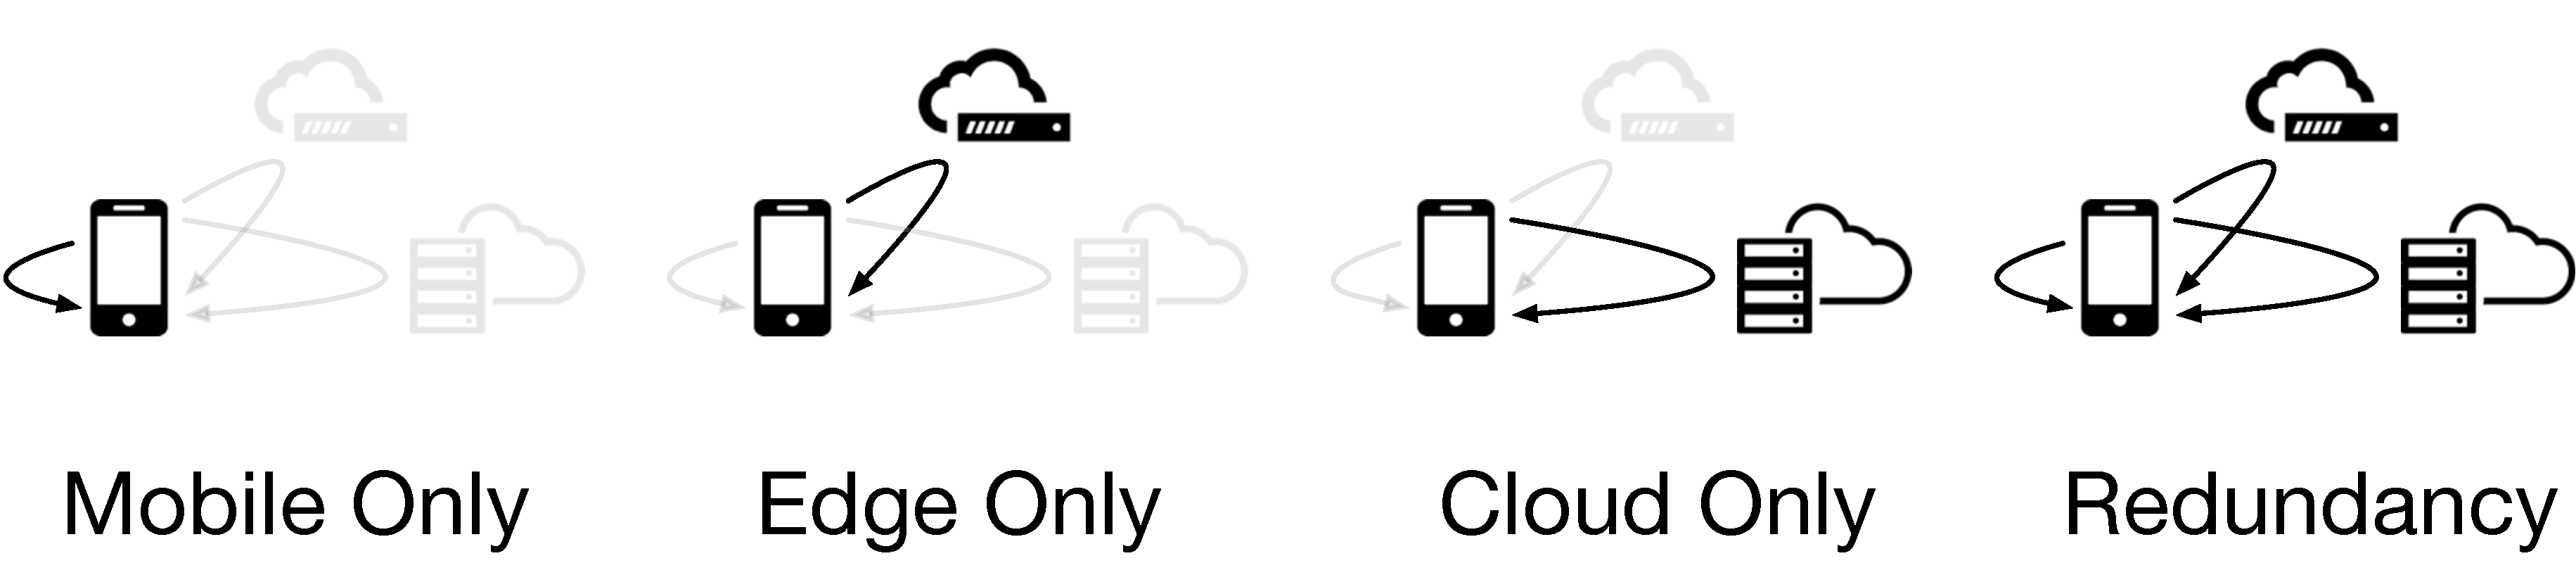
\includegraphics[width=\columnwidth]{figures/redundancy.pdf}
%   \caption{Redundant requests in \sysname{}}
%   \label{fig:redundant}
% \end{figure}

\begin{table*}
  \centering
  \begin{tabular}{c c c c c c}
    \toprule
    Task          & RPi              & Mac             & Swarmbox        & Workstation    & GPU \\
    \midrule
    Encode (JPEG) & 19.6 $\pm$ 2.6   & 4.3 $\pm$ 1.0   & 5.2 $\pm$ 0.9   & 1.3 $\pm$ 0.3  & -   \\
    Decode (JPEG) & 5.4 $\pm$ 0.9    & 1.0 $\pm$ 0.3   & 0.9 $\pm$ 0.2   & 0.5 $\pm$ 0.3  & -   \\
    Viola Jones   & 343.4 $\pm$ 69.4 & 40.0 $\pm$ 10.7 & 48.2 $\pm$ 10.6 & 26.4 $\pm$ 5.7 &     \\
    \bottomrule
  \end{tabular}
  \caption{Performance of analytics operations (serialization, deserialization,
    network transmit, server processing).}
  \label{tab:perf-motiv}
\end{table*}

Our target application environment consists of machines with large range of
computing resources. $(i)$ End-devices, like mobile phones or IoT platforms, are
significantly limited in their computing power. Performing ML inference often
take seconds to complete. $(ii)$ Edge and Cloud. Both the edge and the cloud
suffers from variable latency, unstable connection, and service contention to
provide consistent response times, especially for 99\% requests.

There is a dizzying array of platforms ranging from \$5 Raspberry Pi to \$1000+
GPU-powered workstation~\cite{zhang2015cloud}.  Even in the cloud, there are
various VM options in the cloud: companies rent VMs based on budget or because
of a lack of expertise.

\textbf{Solution:} Because of the such heterogeneity, we hypothesis an ensemble
of available resources (\autoref{fig:dr}) can overcome the shortcomings of
individual platforms and offer end-users with bounded response times, similar to
prior solutions in both cloud-offloading (Tango~\cite{gordon2015accelerating})
and straggler mitigation in the cloud
(Dolly~\cite{ananthanarayanan2013effective}).

\subsubsection*{Network Variations}

\begin{figure}[t]
  \begin{subfigure}[t]{0.49\columnwidth}
    \centering
    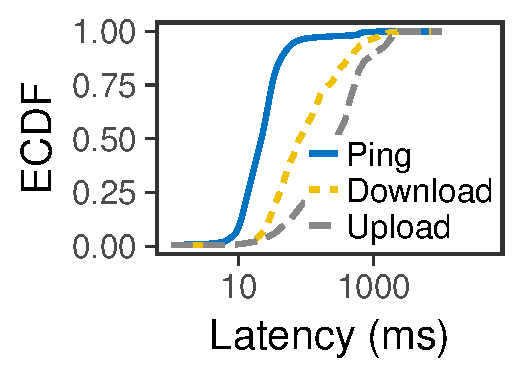
\includegraphics[width=\textwidth]{figures/fcc_latency.pdf}
    \caption{Network latency variation.}
    \label{fig:fcc-latency}
  \end{subfigure}
  \hfill
  \begin{subfigure}[t]{0.49\columnwidth}
    \centering
    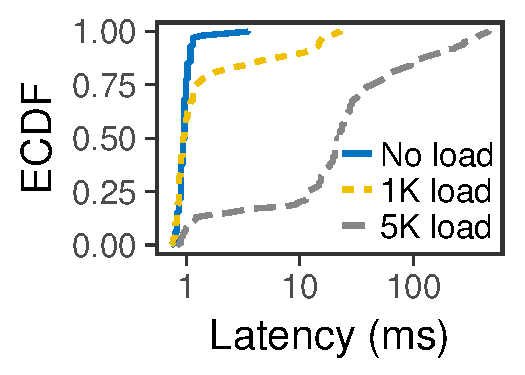
\includegraphics[width=\textwidth]{figures/tf_latency.pdf}
    \caption{Service latency variation.}
    \label{fig:tf-latency}
  \end{subfigure}
  \caption{Network latency increases during downstream and upstream speed tests
    (left). Service time increases during load increase (right).}
\end{figure}

Using FCC broadband measurements, we validate the large variation in wide area
network~(\autoref{fig:fcc-latency}). The median network delay increases from
\SI{22}{\ms} to \SI{80}{\ms} under downstream load and \SI{272}{\ms} under
upstream load.

\textbf{Solution:} Client side, redundant as described above. Server side, time
synchronization and update SLO; and early rejection.

\subsubsection*{Service/Workload Variation}

\noindent We measure TensorFlow serving's performance with different level of load and
validate the large variation in prediction serving
systems~(\autoref{fig:tf-latency}). With modest 1K load, the p99.9 latency
increases from \SI{3.5}{\ms} to \SI{22.5}{\ms}. With 5K load, even the median
latency increases to \SI{21.5}{\ms}: a 22.4$\times$ increase from \SI{0.96}{\ms}
with no load.

\textbf{Solution:} SLO-aware scheduling and the ability to reject requests.

\subsubsection*{Complex Performance Model}

\begin{figure}[t]
  \centering
  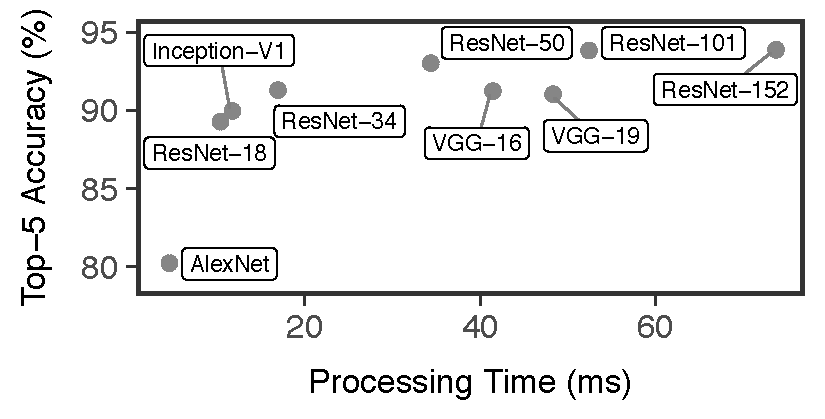
\includegraphics[width=.9\columnwidth]{figures/tradeoff-cnn.pdf}
  \caption{Accuracy-cost trade-off for different CNNs.}
  \label{fig:tradeoff-cnn}
\end{figure}

\begin{figure}[t]
  \centering
  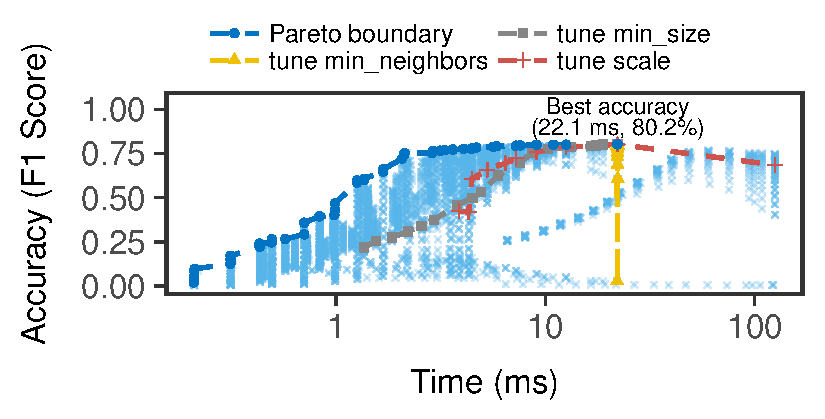
\includegraphics[width=.9\columnwidth]{figures/exhaustive-face.pdf}
  \caption{Complex performance model: spanning multiple dimensions and
    exhibiting non-linear relationship.}
  \label{fig:complex-perf-model}
\end{figure}

For many ML inference task, there exist more than one algorithm, or tunable
parameters for each algorithm with different accuracy and processing times.  We
can speed up computation by providing a less accurate response. This would allow
some computation tractable on end devices and handling more requests on the
edge/cloud.

For example, accuracy-cost trade-offs for object detection using convolutional
neural network (CNN)~\cite{huang2016speed}. \autoref{fig:tradeoff-cnn} shows one
such benchmark~\cite{cnn.benchmarks}.

Many algorithms have large number of knobs to tune that will affect accuracy and
processing cost. We use Viola-Jones (VJ) cascade face
detector~\cite{viola2001rapid} as an example. \autoref{fig:complex-perf-model}
shows the large parameter space with respect to three parameters:
\texttt{min\_size}, \texttt{min\_neighbors}, and \texttt{scale}.

ML algorithms have many tunable parameters. For many algorithms, processing
times and the accuracy may exhibit \textit{non-linear} behavior with respect to
the parameters.

\textbf{Solution:} Bayesian Optimization.

% \begin{table}
%   \small
%   \centering
%   \begin{tabular}{c c c c}
%       \toprule
%       Algorithm & Mobile & Server & GPU \\
%       \midrule
%       VJ Face & $2263.71$ & $197.77 \pm 10.56$ & $23.44 \pm 5.23$ \\
%       HOG + SVM & 1987.9 & 59.7 & 20 \\
%       CNN & $800$ & $300$ & $40$ \\
%       \bottomrule
%     \end{tabular}
%    \caption{Processing Times for Example Model Serving on different
%      platforms.\protect\footnotemark}
%    \label{tab:times}
% \end{table}

% \footnotetext{Mobile is Android Nexus 7; Server is Intel Core XXX; GPU is GTX
%   970. Data is averaged over 100 frames with resolution $640 \times 480$.}

%%% Local Variables:
%%% mode: latex
%%% TeX-master: "../serving"
%%% End: